\documentclass[11pt,a4paper]{article}

% Compile with LuaLaTeX. The page geometry, type size, spacing, and headings
% are chosen to make page density close to the corresponding Word template, 
%so that the length of reports is the same regardless of which template is used.

\usepackage[margin=1in,headheight=15pt,headsep=24pt,footskip=28pt]{geometry}
\usepackage[default]{sourcesanspro}
\usepackage{setspace}
\usepackage{xcolor}
\usepackage{mdframed}
\usepackage{titlesec}
\usepackage{fancyhdr}
\usepackage{lastpage}
\usepackage{microtype}
\usepackage{graphicx}
\usepackage{booktabs}
\usepackage[hidelinks]{hyperref}
\usepackage[numbers,sort&compress]{natbib}
\renewcommand{\bibsection}{\unnumberedheading{\refname}}

\definecolor{guidancetext}{HTML}{595959}
\definecolor{guidancebg}{HTML}{F1F3F5}

\setstretch{1.5}
\setlength{\parindent}{0pt}
\setlength{\parskip}{10pt}
\raggedbottom

\titleformat{\section}
  {\fontsize{14}{16.5}\selectfont\bfseries}
  {\thesection}{1em}{}
\titlespacing*{\section}{0pt}{0pt}{12pt}
\titleformat{\subsection}
  {\fontsize{13}{15.5}\selectfont\bfseries}
  {\thesubsection}{1em}{}
\titlespacing*{\subsection}{0pt}{0pt}{4pt}

\newcommand{\unnumberedheading}[1]{%
  \par\vspace{2pt}{\fontsize{14}{16.5}\selectfont\bfseries #1\par}\vspace{6pt}%
}
\newcommand{\reporttitle}[1]{%
  {\fontsize{16}{19}\selectfont\bfseries #1\par}\vspace{12pt}%
}
\newcommand{\guidance}[1]{%
  {\setstretch{1.0}\fontsize{9}{11}\selectfont\color{guidancetext}\itshape #1\par}%
  \vspace{-6pt}%
}
\newenvironment{guidancebox}
  {\begin{mdframed}[backgroundcolor=guidancebg,linecolor=guidancebg,linewidth=0pt,
    innerleftmargin=3pt,innerrightmargin=3pt,innertopmargin=2pt,innerbottommargin=2pt,
    skipabove=6pt,skipbelow=10pt]
   \setstretch{1.0}\fontsize{9}{11}\selectfont\color{guidancetext}\itshape\setlength{\parskip}{6pt}}
  {\end{mdframed}}
\newcommand{\placeholder}[1]{#1\par}

\pagestyle{fancy}
\fancyhf{}
\renewcommand{\headrulewidth}{0pt}
\renewcommand{\footrulewidth}{0pt}
\fancyhead[L]{\fontsize{9}{11}\selectfont II2202, Autumn 2026, Period 1}
\fancyhead[C]{\fontsize{9}{11}\selectfont Research plan}
\fancyhead[R]{\fontsize{9}{11}\selectfont 11 September 2026}
\fancyfoot[R]{\fontsize{8.5}{10}\selectfont \thepage\ (\pageref{LastPage})}

\begin{document}
\reporttitle{Transparent Multi-Hop Routing for Raft Under Partial Network Partitions}
\unnumberedheading{Authors}
Lorenzo Deflorian <ldef@kth.se>\par
Juozas Skarbalius <juozas@kth.se>\par
\vspace{2pt}

\unnumberedheading{Abstract}
Distributed systems utilize consensus protocols to find agreement on a shared state. 
Raft - one of such protocols - is a leader-based consensus protocol.
In order for Raft to make progress, it needs to be able to communicate with a majority quorum via P2P links. 
However, in partial network topologies, some of the links may fail, causing the leader to lose contact with such quorum.
In this case, the leader may not be able tocontinue making progress, and in certain topologies, unable to elect next leader.

One of the proposed solutions to this problem by the state-of-the-art is to use network overlays on top of the existing consensus protocol.
However, such solution is not sufficiently evaluated by prior work in the context of Raft.
This research plan proposes to evaluate the effect of multi-hop routing on Raft's liveliness and latency.

\section{Introduction}

\subsection{Background and Rationale}

Various distributed systems, such as databases, distributed file systems, and cluster membership frameworks, rely on consensus protocols to find agreement on a shared state. 
Raft is a leader-based consensus protocol in which the leader appends client entries to its log and replicates them to its followers. 
An entry can be committed once it has been replicated to a majority of the nodes~\cite[Sec.~5.3]{ongaro2014raft}. 
The protocol remains safe under arbitrary message delay and can continue to make progress while a leader can communicate with a majority of the nodes~\cite[Secs.~5.3--5.4]{ongaro2014raft}.

The consequences of a complete network partition are well understood in majority-based consensus. 
If a minority of nodes becomes unreachable, the remaining majority can continue to make progress. 
A group that cannot communicate with a majority cannot commit new entries. 
Partial network partitions present a different challenge: some direct links between nodes fail even though the nodes remain connected through intermediate nodes~\cite[Sec.~2]{alfatafta2020nifty}.

Raft's communication model assumes direct point-to-point exchanges between participating nodes and does not provide multi-hop forwarding~\cite[Secs.~5.1--5.3]{ongaro2014raft}. 
A leader that loses direct contact with two followers may therefore be unable to form a quorum, even if both followers could still be reached through another replica at the network layer. 
The mismatch between indirect paths between nodes being available and the Rafts inability to utilize such paths motivates studying whether transparent multi-hop routing can restore Raft progress and under what cost.

\subsection{Theory and Related Work}

Prior work has examined partial network partitions from several angles. 
Jensen et al.~\cite[Sec.~4, Figs.~5--9]{jensen2021raft} studied etcd's Raft implementation under partial network failures. 
Their experiments demonstrate election instability and delayed requests in several partition scenarios. 
They identify overlay networks as a possible solution that could reroute traffic between two replicas through a third, but do not implement or evaluate that approach for Raft~\cite[Sec.~5]{jensen2021raft}.

Alfatafta et al.~\cite[Sec.~6]{alfatafta2020nifty} introduced Nifty, a transparent communication layer that monitors connectivity and detours packets around failed paths through bridge nodes. 
Their evaluation shows that Nifty can mask partial partitions with low failure-free overhead in six systems~\cite[Secs.~7.1--7.2]{alfatafta2020nifty}. 
However, the evaluated systems do not include a Raft deployment, so the study does not establish when routed paths restore Raft progress or how added path delay affects Raft commit latency.

Omni-Paxos takes a different approach by changing the consensus protocol itself to handle partial connectivity. 
Ng et al. analyze how established leader-based protocols can deadlock or livelock when no suitable leader can be elected or maintained despite residual network connectivity~\cite[Sec.~2, p.~117]{ng2023omnipaxos}. 
They define quorum-connected leader election and separate leader election from log replication so that leader selection can focus on connectivity~\cite[Sec.~5.1, p.~121]{ng2023omnipaxos}. 
The authors also discuss transparent overlay routing as a general alternative, but argue that extra hops and network delays may reduce fault tolerance and performance~\cite[Sec.~8, p.~127]{ng2023omnipaxos}. 

Together, these studies establish that partial connectivity can disrupt Raft-like protocols and that transparent routing can mask partial partitions in other systems. 
They do not, however, provide an experimental characterization of the topologies in which transparent multi-hop routing restores Raft progress or of the commit-latency cost when routed followers are needed to form a quorum. 
This missing evaluation is the research gap that will be addressed by this proposed study.

\subsection{Research Problem, Aim, and Research Questions}

\textbf{Research problem.}
Existing work establishes that Raft can lose liveness or experience election instability under partial connectivity~\cite[Sec.~4]{jensen2021raft}. 
Nifty demonstrates that transparent multi-hop routing can mask partial partitions without changing the application~\cite[Secs.~6--7]{alfatafta2020nifty}, and similar routing has been proposed as a possible solution for Raft~\cite[Sec.~5]{jensen2021raft}. 
However, the liveness benefit and commit-latency cost of applying such routing to Raft have not been experimentally characterized.

\textbf{Aim.}
We aim to experimentally characterize transparent multi-hop routing as a network-layer resilience mechanism for Raft under a defined set of partial-connectivity topologies, in terms of liveness and commit latency, without changing the consensus implementation itself.

\textbf{Objectives.}
During the course project, we will:
\begin{enumerate}
  \item construct controlled Raft configurations of five and three nodes that can reproduce a healthy baseline and four predefined partial-connectivity topologies;
  \item compare direct communication with transparent multi-hop routing using repeated trials and take measurements of commit progress, recovery time, number of elections and their stability, and the number ofterm changes;
  \item measure client-side commit latency in all scenarios
  \item document the implementation, experiment, and results required to reproduce the study.
\end{enumerate}

\textbf{Research questions.}
\begin{enumerate}
  \item \textbf{RQ1 (Liveness):} Across the predefined T1--T4 partial-connectivity topologies---a non-critical cut, quorum-loss, constrained election, and chained connectivity---in which cases does transparent multi-hop routing restore stable Raft progress compared with direct communication only?
  \item \textbf{RQ2 (Latency):} How does added per-link delay on transparent multi-hop paths affect client-observed Raft commit latency when a follower reached through such a path belongs to the deciding majority?
\end{enumerate}

\textbf{Hypotheses.}
We expect transparent forwarding to restore progress in the tested topologies where the routed graph gives a viable leader stable bidirectional paths to a majority (H1). We expect commit latency to increase with the additional round-trip delay of a forwarded path when a follower on that path is required to complete the deciding majority, while little or no increase is expected when the leader retains a sufficient direct quorum (H2).

\section{Research Method}

\subsection{Research Design and Methodological Rationale}

We plan to answer both research questions through quantitative experiments in an emulated network. 
For each topology and delay, both communication modes (i.e., direct point-to-point and multi-hop forwarding) will use the same Raft implementation, failed links, workload, and configuration. 
Repeating the same conditions will help account for variation in election timing, message scheduling, and host load.

For RQ1, we will observe whether Raft maintains or recovers stable commit progress in each topology. 
T0 provides a healthy baseline, while T1 is a control case in which the leader keeps a direct quorum after a link failure. 
T2--T4 represent the quorum-loss, constrained-election, and chained-connectivity failures. 
Running each scenario with and without forwarding will show in which cases forwarding restores progress.

For RQ2, we will repeat the comparisons with per-link delays of 0.5, 5, and 20\,ms. 
We will then compare the client-side commit latency when a forwarded path is needed to form the deciding majority. 
T1 also provides a useful control for this question because the leader can still form a majority through direct links.

We decided not to use the Nifty implementation. 
Its failure detection and route discovery would make it harder to separate the effect of multi-hop communication from the time needed to discover and install a route. 
Instead, we will preconfigure Linux forwarding and focus on the effect of path availability and delay.

We also considered hosting the experiment in the cloud (e.g., AWS or GCP). 
However, due to time constraints of this course, we opted for using our personal machines instead.
We intend to host multiple node instances and virtual network infrastructure implementing each topology on our machines.

\subsection{Experimental Platform, Conditions, and Evidence}

We plan to use HashiCorp implementation of Raft~\cite{hashicorp_raft}. 
If additional measurement instrumentation is needed, it will be documented and applied in the same way in both modes.

We plan to build the network using Mininet 2.3.0~\cite{lantz2010mininet,mininet230}. 
Each Mininet host will run one Raft replica with a stable address. 
Mininet will create the links, apply delay, and inject the planned link failures. 
In direct-only mode, Raft nodes will only communicate over their surviving direct links. 
In forwarding mode, preconfigured Linux routes and IP forwarding will carry the same traffic through intermediate nodes. 
Raft will continue to use the same peer addresses in both modes.

The complete experiment will run on a standard Linux virtual machine. 
The exact processor, number of virtual CPUs, amount of memory, Linux distribution, and kernel version have not yet been selected. 
We will fix and report these details before running the main experiments. 
We will also monitor the host load to check that competition for resources does not dominate the results.

Figure~\ref{fig:topologies} shows the five topologies that we plan to test. 
All links in the figure are bidirectional. 
T0 uses five fully connected nodes and provides the healthy baseline. 
T1 removes the link between C and E, but leader C can still communicate directly with a majority.

T2 uses five nodes with A as the only node connected directly to a majority. 
The initial leader C can reach A but cannot reach a majority directly. 
T3 isolates the initial leader C, while A remains connected to B, D, and E. 
The initial logs are A=$[1,1]$, B=$[1,1,2]$, C=$[1,1,2,2]$, D=$[1,1,2]$, and E=$[1,1]$. 
This makes A the only quorum-connected candidate, although B and D have newer logs.

T4 uses three nodes connected as the chain B--A--C, with B as the initial leader and no direct link between B and C. 
This is the chained scenario evaluated by Ng et al.~\cite[Sec.~7.2, pp.~124--126]{ng2023omnipaxos}. 
In forwarding mode, B and C will communicate through A without adding or repairing a physical link.

What we vary is the communication mode, the topology, and the per-link delay. 
We will collect client request and commit timestamps, commit latency, recovery time, commit throughput over time, and leader and term changes. 
One open-loop client will submit requests independently of the completion of previous requests. 
The request rate, entry size, timeout, and exact schedule will be fixed after the pilot and then kept the same for all main runs. 
Client-side timestamps will record submissions and commit confirmations, while Raft event records will provide information about leaders, terms, and commits. 
During the initial experiment, we will determine whether the existing logs and observer interfaces provide all the required information or whether additional instrumentation is needed.

The planned evaluation contains five topologies, two communication modes, three delay settings, and 20 repetitions of each condition. 
This gives a target of 600 runs. 
We will first automate five pilot runs for each condition to estimate the variability and total running time. 
Based on the initial experiments, we will confirm whether 20 repetitions are feasible or adjust the number before collecting the remaining data. 

The study does not involve human participants or collection of personal or sensitive data, and all required software is open source. 
Therefore, we do not expect any participant-related ethical issues or any need to purchase data. 

\begin{figure}[p]
  \centering
  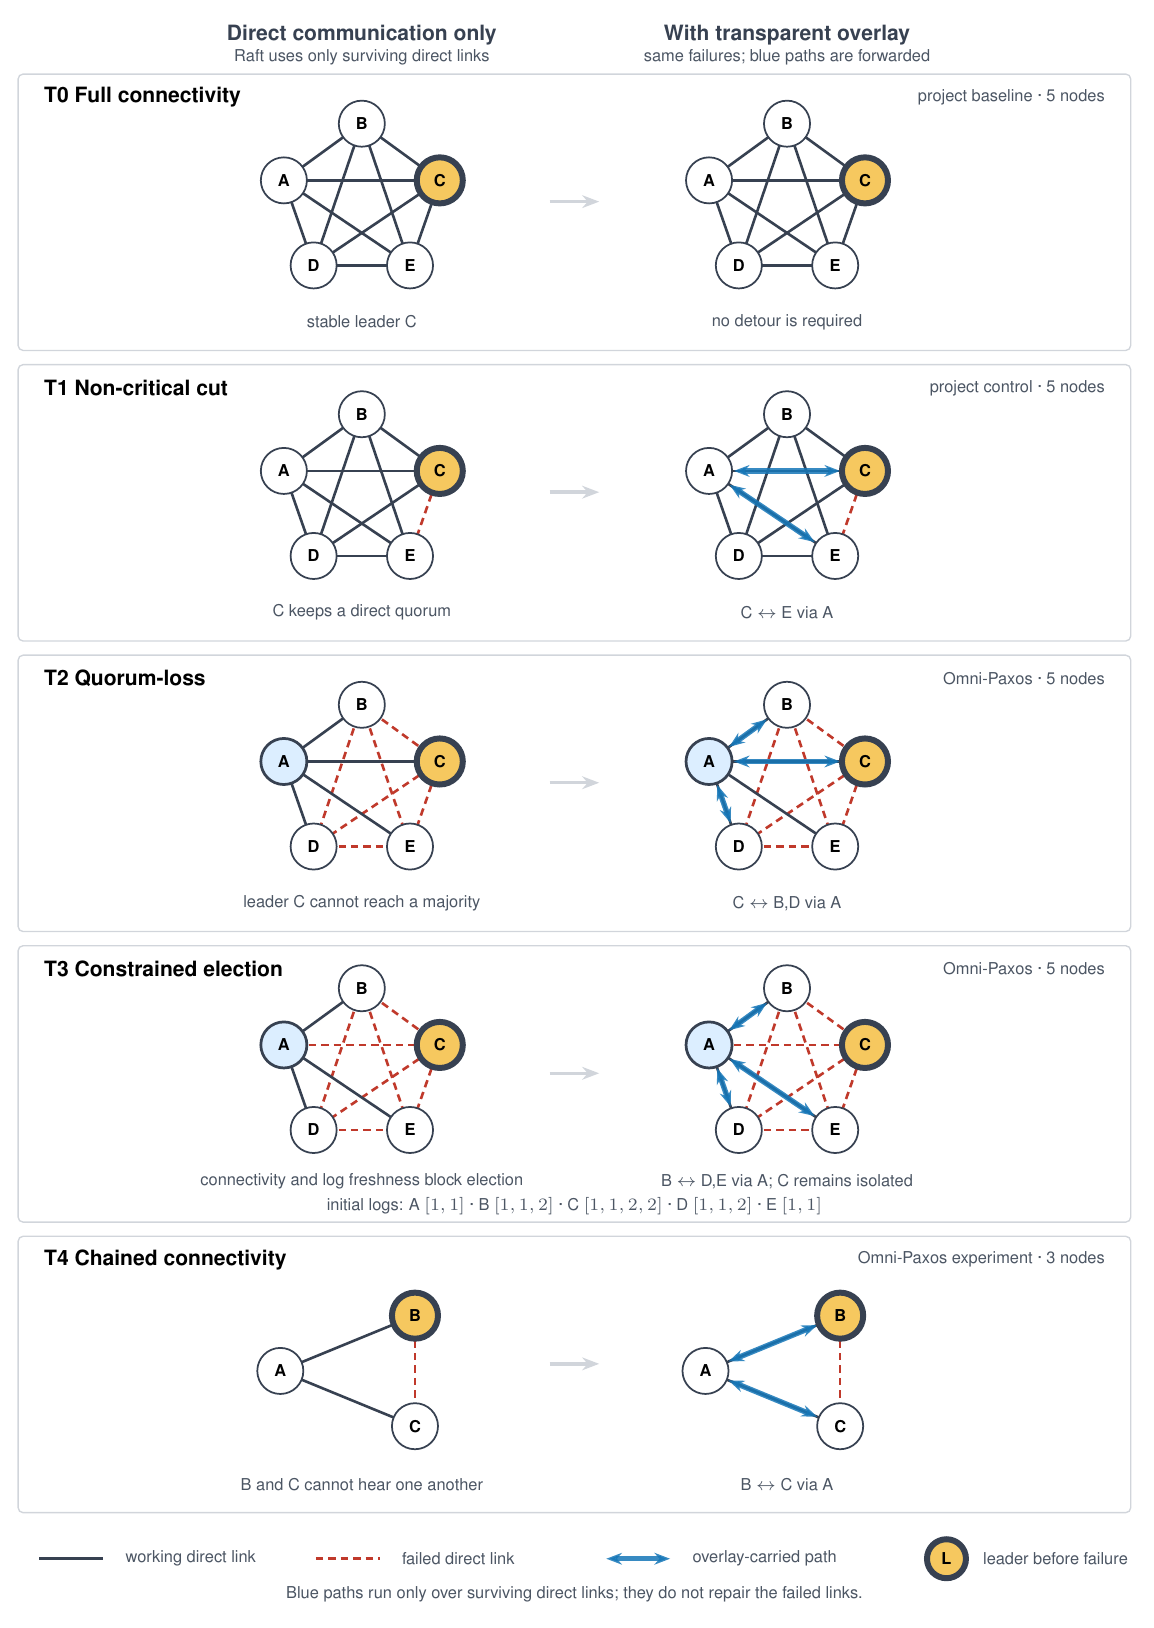
\includegraphics[width=0.94\textwidth]{figures/topology-scenarios.png}
  \caption{Planned direct-only and transparent-forwarding conditions. Solid links remain available, dashed links have failed, and blue paths show forwarding over surviving links.}
  \label{fig:topologies}
\end{figure}
\clearpage

\subsection{Work Procedure and Data Collection}
Before defining the experiment procedure, we will first define the variables that we control (independent variables) and the variables that we attempt to measure (dependent variables).
Tables~\ref{tab:independent-variables} and~\ref{tab:dependent-variables} summarize these variables and their levels or definitions.

\begin{table}[htbp]
  \centering
  \caption{Independent variables.}
  \label{tab:independent-variables}
  \begin{tabular}{ll}
    \toprule
    Independent variable & Level \\
    \midrule
    Communication mode & Point-to-Point (P2P) RPC, Multi-hop RPC forwarding \\
    Topology & T0--T4 \\
    Per-link delay & 0.5, 5, 20\,ms \\
    Raft heartbeat interval & 1, 10, 500\,ms \\
    \bottomrule
  \end{tabular}
\end{table}

\begin{table}[htbp]
  \centering
  \caption{Dependent variables.}
  \label{tab:dependent-variables}
  \begin{tabular}{lll}
    \toprule
    Dependent variable & RQ & Definition \\
    \midrule
    Commit throughput & RQ1 & Committed and appended entries per second \\
    Recovery time & RQ1 & Time from failure to first subsequent commit \\
    Number of elections & RQ1 & Count during the observation window \\
    Number of term changes & RQ1 & Count during the observation window \\
    Commit latency & RQ2 & Client request-response delay \\
    \bottomrule
  \end{tabular}
\end{table}

Each experiment for a set of independent variables will proceed as follows:
\begin{enumerate}
  \item Start a clean Mininet topology for the chosen T0--T4 scenario and apply the chosen per-link delay to all surviving links.
  \item For each communication mode (P2P and multi-hop forwarding) and repeat 20 times:
  \begin{enumerate}
    \item Configure and start the Raft replicas with the planned initial leader and heartbeat interval.
    \item Start the open-loop client.
    \item Wait for couple of seconds and verify that the cluster is initially healthy and commits are succeeding.
    \item Induce partial network partitions by failing previously planned links of the current tested topology.
    \item Stop the client and replicas, archive all logs and measurement files under a unique run identifier, and tear down Mininet before the next run.
  \end{enumerate}
\end{enumerate}

\textbf{Data collection.}
Client-side records will store request identifiers, submission timestamps, and commit-confirmation timestamps.
Raft event records will store leader identity, term changes, and commit events, election timestamps.
All raw outputs will be written to files named by condition and repetition so that they can be joined into a single analysis dataset without manual transcription.

\subsection{Data Analysis and Quality Assurance}

\textbf{RQ1 analysis.}
For each topology and communication mode we will classify a run as making stable progress if the cluster commits new entries throughout the post-failure observation window after at most a bounded recovery period, without sustained election churn.
We will report the fraction of runs that meet this criterion, the distribution of recovery times among successful recoveries, and summary counts of elections and term changes.
The primary comparison is direct-only versus forwarding within each topology.
T0 and T1 serve as sanity checks: both modes should remain live in T0, and direct-only should already remain live in T1.
Answers to RQ1 will therefore be stated as the set of topologies among T2--T4 in which forwarding restores stable progress relative to direct-only communication under the same delay and workload.

\textbf{RQ2 analysis.}
For each completed request we will compute commit latency from the client timestamps.
We will summarize latency with the median and selected upper percentiles (for example, the 95th percentile) within each condition, and we will compare forwarding against direct-only at each delay setting.
The analysis will distinguish cases in which a forwarded follower is required to form the deciding majority from control cases such as T1, where the leader retains a direct quorum.
If forwarding restores progress in a topology where direct-only does not, the latency characterization for that topology will be reported for the forwarding mode alone, together with the corresponding path delay.
We will use non-parametric comparisons across repeated runs (for example, Wilcoxon rank-sum tests on per-run median latency, with effect sizes) rather than relying only on visual inspection, and we will report confidence intervals for the main latency summaries.

\textbf{Threats to validity and mitigation.}
Election timing, message scheduling, and host contention introduce run-to-run variability that could obscure the effect of forwarding or delay.
We will mitigate this by repeating each condition, recording seeds, running trials sequentially, and monitoring host load against a predefined overload threshold.
Configuration errors could allow traffic to bypass a failed link or prevent a planned forwarded path from working; batch-level connectivity and delay checks, together with predefined exclusion and rerun rules, are intended to limit such contamination.
Measurement clock skew between client timestamps and Raft logs could distort latency if clocks are not aligned; we will prefer client-side submission and confirmation timestamps for RQ2 and cross-check commit events against Raft records for consistency rather than mixing clocks unnecessarily.
Implementation-specific behaviour in HashiCorp Raft may differ from Raft theoretical model; we will document the library version and configuration, and we will treat unexpected negative findings as results rather than altering topologies after data collection.
External validity is limited to the emulated Mininet setting, the chosen topologies, and the selected delays; we will state these bounds explicitly when interpreting the results.

\textbf{Reproducibility.}
We will publish or archive the experiment scripts, topology definitions, forwarding rules, workload parameters, seeds, raw measurement files, and analysis notebooks used to produce the reported figures and tables.
The final report will list the virtual-machine specification, Linux distribution and kernel version, Mininet version, HashiCorp Raft version, and any instrumentation added for measurement.
Together with the fixed trial sequence above, this material is intended to make the study reproducible by an independent party on equivalent hardware.

\subsection{Use of AI Tools}
AI tools will be used to assist with writing helper and configuration scripts for the experiments, as well as for checking and correcting the text in report drafts and final report in terms of grammar and style.
AI-produced content will be verified and checked by us.

\section{Project Planning and Feasibility}

\subsection{Work Tasks and Milestones}

The work will be divided into five ordered stages. We do not assign calendar dates at this point, but each stage ends with a milestone that must be completed before the dependent work begins.

\textbf{Stage 1: Finalize the experimental protocol.}
We will define the remaining workload parameters, trial timing, measurement rules, and exclusion criteria. We will also fix the virtual-machine configuration and record the software and system settings. The first milestone is a complete experiment specification that can be applied without making new decisions during data collection.

\textbf{Stage 2: Build and validate the testbed.}
The HashiCorp Raft cluster, open-loop client, Mininet topologies, forwarding rules, failure injection, and data collection will be implemented. Unit-level checks will first verify the individual components. The components will then be combined in the three-node forwarding cluster. The second milestone is a testbed that reproduces the planned direct-only and forwarding conditions and records the required measurements.

\textbf{Stage 3: Conduct the initial experiments.}
We will automate five pilot runs for every experimental condition. The initial experiments will be used to detect implementation problems, estimate variability and total running time, and decide whether the target of 20 repetitions remains feasible. Any resulting changes will be made before the procedure is frozen. The third milestone is a validated final procedure and a justified repetition count.

\textbf{Stage 4: Collect and analyze the main data.}
We will execute the remaining runs in batches. Connectivity, delay, and host load will be checked for every batch, and each run will retain its configuration and random seed. After validating the collected data, we will analyze liveness and recovery for RQ1 and commit latency for RQ2. The fourth milestone is a complete, quality-checked dataset with results for both research questions.

\textbf{Stage 5: Report and reproduce the study.}
We will interpret the results, discuss limitations and alternative outcomes, and complete the final report. The final milestone is a final report.

\subsection{Allocation of Responsibilities}

The implementation work will be divided into two connected parts. 
Lorenzo will lead the Raft, client-workload, and measurement components. 
Juozas will lead the Mininet topologies, routing configuration, delay control, and failure injection. 
Each person will review and test the other part before the components are combined. 
Experiments will be either conducted jointly, or independently, and then analyzed, reviewed and discussed together.

The analysis will also be divided while keeping both group members involved. 
Lorenzo will lead the liveness, recovery, and election analysis for RQ1. 
Juozas will lead the commit-latency analysis for RQ2. 
Both will inspect the complete set of metrics and other data collected, 
verify the analysis produced by the other person, and interpret the results together. 

Writing will follow the same division for the first drafts, while the research method, discussion, conclusions, and final revision will be completed jointly. 
Progress will be tracked via regular short meetings, and shared issues in the project repository. 
All code and report changes will be reviewed by the other group member. 
Both authors will therefore remain able to explain the experimental setup, analysis, and conclusions.

\subsection{Implementational Risks and Mitigation Strategies}

\textbf{Incorrect network isolation or forwarding.}
A configuration error could allow traffic to bypass a failed link or prevent a planned forwarded path from working. We will first test the three-node chained topology and verify reachability and end-to-end delay before every experimental batch. If a validation fails, the batch will not begin until the routes and failure rules have been corrected. Runs affected by an undetected configuration error will be excluded according to a predefined rule and repeated from a clean state.

\textbf{The expected Raft failure does not appear.}
HashiCorp Raft may behave differently from the protocol model because of its implementation details or election timing. We will verify the initial leader, connectivity, and log state before injecting each failure, and we will use repeated runs and recorded seeds to distinguish consistent behaviour from timing variation. If a topology still does not produce the expected failure after the setup has been validated, the result will be reported as a negative finding rather than changing the topology after data collection.

\textbf{Host contention affects the measurements.}
Running all replicas, the client, and Mininet on one virtual machine may introduce CPU or memory contention that hides the effect of network delay. We will run trials sequentially, keep the VM configuration fixed, and monitor host load. We will define an overload threshold before the main experiment. If a batch exceeds this threshold, we will move to a larger VM or reduce the offered workload and repeat the complete affected batch under one fixed configuration.

\bibliographystyle{myIEEEtran}
\bibliography{II2202-research-plan}
\end{document}
